\documentclass[letterpaper,oneside]{scrartcl}
\usepackage{fullpage}
\usepackage[utf8]{inputenc}
\usepackage[pdftex]{graphicx}
\DeclareGraphicsExtensions{.png,.pdf}
\graphicspath{{plots/}}
\usepackage{hyperref}
\usepackage{url}
\usepackage[round,sectionbib]{natbib}
\bibliographystyle{abbrvnat}
\usepackage[small]{caption2}
\usepackage[small]{titlesec}
\renewcommand\familydefault{bch}

\title{Product graphics}
\author{Hadley Wickham and Heike Hofmann}
\begin{document}
\maketitle
  
\section{Introduction}

% JASA methods
% Infovis?

% Aims of this paper:
%
%  * emphasise the connection between area products and factorising 
%    probabilities
% 
%  * pull all area plots on a common footing - provide a grammar for 
%    categorical graphics

Area plots are the graphical equivalent of contingency tables, displaying how a total is broken down into components.  

display categorical data with a rectangle for each combination of the factors of interest, with the area of the rectangle proportional to the number of observations in that combination. 

The layout of the rectangles give rise to the difference categorical plots that we are familiar with: bar charts, spine charts, mosaic plots \citep{hartigan:1984,hartigan:1981,friendly:1994,hofmann:2003},  equal-bin-size plots, and fluctuation diagrams. Trellis graphics are another type of display that uses categorical variables to create small multiples for different subsets of the data. Visually, trellis graphics look like equal-bin-size plots with another plot drawn inside each bin. 

Figure \ref{fig:cat-examples} illustrates some of these plots.

\begin{figure}[htbp]
  \begin{center}
  %  \includegraphics[scale=1]{file}
  \end{center}
  \caption{Area plot examples.}
  \label{fig:cat-examples}
\end{figure}

Hierarchical partitioning of space.

Basic idea is factorising table of probabilities:

\begin{itemize}
  \item as products of marginal and conditional distributions
  \item as areas in plots
  \item as sums of parameters in log-linear models
\end{itemize}

Let $f(x, y, z)$ be the 3d pmf function.  We can can write this pmf as product of marginals and conditionals in many different ways.  We can decompose product graphics in a similar way.

\begin{itemize}
  \item $f(x, y, z) = f(x, y | z) f(z)$
  \item $f(x, y, z) = f(x | y, z) f(y, z)$
  \item $f(x, y, z) = f(x | y, z) f(y | z) f(z)$
\end{itemize}

These techniques are also closely related to dimensional stacking \citep{leblanc:1990}

% Other papers to cite:
% 
% Generalised treemaps: \citep{vliegen:2006}
% Cocktailmaps: \citep{ahlberg:1996}
% Extension to mosaic: \citep{friendly:1999,hofmann:2000}
% Connection to models: \citep{theus:1999,hofmann:2001}


% Hierarchical coordinate systems 
%
% What are the common components of all these plots, and how can be describe
% them in a succinct way that also allows us to describe what tasks each
% display is good for?  We propose that there is one key feature that makes
% these plots special.  That is there their coordinate system, which is
% hierarchical.  
%
% In most coordinate systems that we are used to, such as Cartesian or polar
% coordinates, are symmetric in the sense that you can locate a point by
% starting from either dimension.  For example, in Cartesian coordinates you
% can identify either the x- or y-coordinate first, and the other next.  This
% also implies a distance symmetry when projected onto 2D Euclidean geometry.
% When you vary one coordinate by a small amount (holding all others constant)
% points in the projective geometry will be close.
%
% Neither of these properties hold for hierarchical coordinate systems. 
%
% We will discuss hierachical coordinate systems in general, and then present
% a specific hierachical coordinate system which gives rise to the area plots
% described previously. 

To illustrate these ideas, we'll use a small sample from the general social survey ({\sc gss}) focussing on happiness. 51\,020 observations from cross-section survey given yearly from 1972 to 2006.

\begin{itemize}
  \item Happy.  Discrete: ``very happy'', ``pretty happy'', ``not too happy''
  \item Age (in years), 18--89.
  \item Sex: ``female'', ``male''
  \item Degree: ``lt high school'', ``high school'', ``junior college'', ``bachelor'', ``gradudate''
  \item Relative financial status {\sf finrela}: ``far above average'', ``above average'', ``average'', ``below average'', ``far below average''
  \item Health: ``excellent'', ``good'', ``fair'', ``poor''
  \item Year: 1972--2006.
  \item Probability weight ({\sf wtsall}): 0.43--6.42.
\end{itemize}


\section{Display}
\label{sec:display}

Perceptual constraints.  Best at comparing area when:

\begin{itemize}
  \item Simple shape (i.e. square vs polygon)
  \item Aspect ratios similar
  \item Areas are large
  \item Areas are close
  \item One border is constant.
\end{itemize}

Impossible to simultaneously satisfy all constraints.  Every product plot requires the creator to trade off between these.  

Constraints on partitioning

\begin{itemize}
  \item Area should be proportional to weight
  \item Containment / Non-overlapping
\end{itemize}

We will add one more constraint to reduce the space of possible

\begin{itemize}
  \item Rectangular partitions
\end{itemize}

We will focus our attention on rectangular partitions.  In general,  $h(i, j) = c(i, j)^x$ $w(i, j) = c(i, j)^y$, $x + y = 1$.   Basic principle of all area plots is area should be proportional to probability. For the plots we are interested in, the shape used to represent the count is a rectangle, so that $a(i, j) = w(i, j) * h(i, j)$.

\subsection{1d primitives}

Space-filling vs. not space-filling.  Read length on common scale, vs. put more information in the display.

Each plot type constrains this relationship in a different way:

\begin{itemize}
  \item {\bf bar}: height is proportional to value, width equally divides space. Bars allow comparison between absolute numbers.

  \item {\bf spine}: width is proportional to value, height equally divides space. Spines not useful at top level, but allow comparison of proportions at next level (ie. conditioned on top level values)

  \item {\bf treemap}: no restrictions on height and width.   At first glance, it may seem strange to include the treemap as a 1d primitive, but it lays out a single variable in 2d dimensions, just like the other approaches.

\end{itemize}

\subsection{2d primitives}


\begin{itemize}
  \item {\bf fluct}: width and height proportional to square root of value. Flucts allow comparisons of absolute numbers in two directions. 
  
\end{itemize}

One special 2d case is the equal bin size plot - which all 1d x 1d primitives and the fluct collapse to when counts are equal. 


\subsection{Plot templates}

Plot templates combine the simple primitives into well-known graphics:

\begin{itemize}
  \item {\bf Stacked} barchart: 1 bar + $n-1$ spines in opposite direction.
  \item {\bf Nested} barchart: $n$ bars.
  \item {\bf Mosaic} plot: spines in alternating directions.  The 1d case has a special name, the spineplot.
  \item {\bf Double-decker} plot: $n-1$ spines + 1 spine in opposite direction.
  
  \item {\bf Fluctuation} diagram: 
\end{itemize}



\subsection{Violation of constraints}

\subsubsection{Area not proportional to weight}

It can be useful to violate the constraint that area should be proportional to weight to distinguish between zeros and very small values.  A zero weight should have zero area, but giving it positive area can be useful so it's actually possible to see!  Similarly for very small values which would otherwise occupy less than a pixel, useful to constain to minimal perceptible size.

Antony's zooming, where you also truncate the maximum size.

Image.

\subsubsection{Overlapping rectangles}

The cascaded treemaps of \citet{lu:2008} is an idea that illustrates how the violation of containment can be productive.  In the cascaded treemap, each level is slightly offset from the one above to create a pseudo-3d perspective.

Example

\subsubsection{Non-rectangular partitions}

Pie charts fall out naturally, as bars in polar coordinates, with angle and radius instead of height and width. And to ensure that counts stay proportional to areas, the square-root is taken of the y-axis. This is related to the infoslices of \citet{andrews:1998}, which only use half of the disk. Figure~\ref{fig:polar} shows some examples of product plots in polar coordinates.

These displays generalise the fourfold displays of \citet{friendly:1995}. 

\begin{itemize}
  \item Pie charts
  \item Nightingale
  \item Bullseye chart 
\end{itemize}

\begin{figure}[htbp]
  \centering
    \includegraphics[width=0.25\linewidth]{hb-vb-cartesian}%
    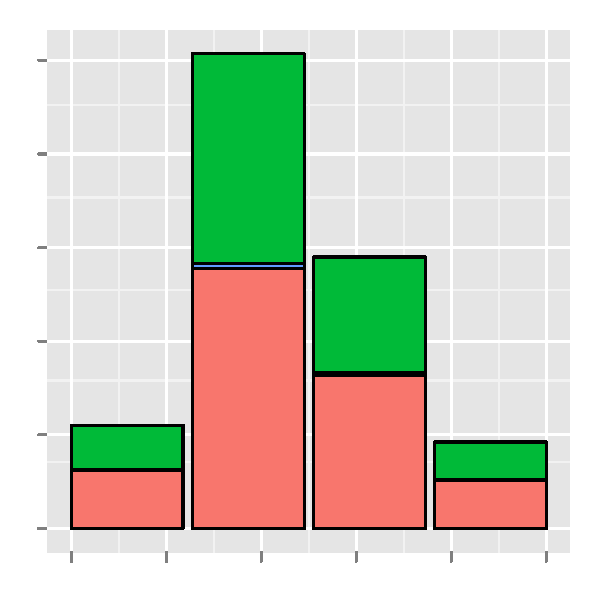
\includegraphics[width=0.25\linewidth]{hb-vs-cartesian}%
    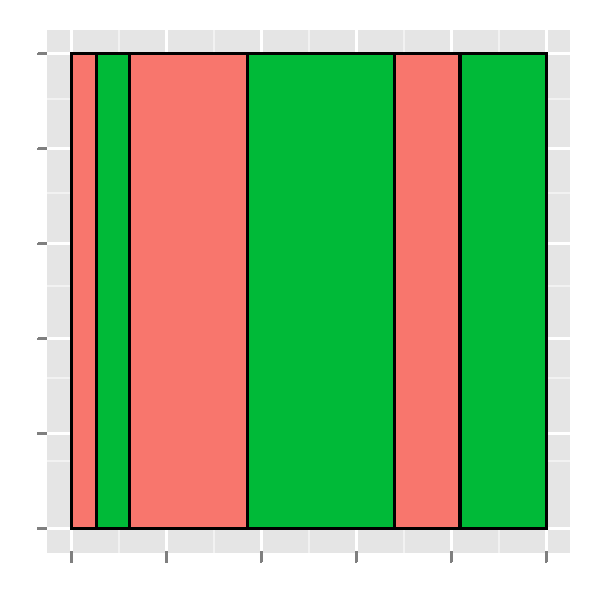
\includegraphics[width=0.25\linewidth]{hs-hs-cartesian}%
    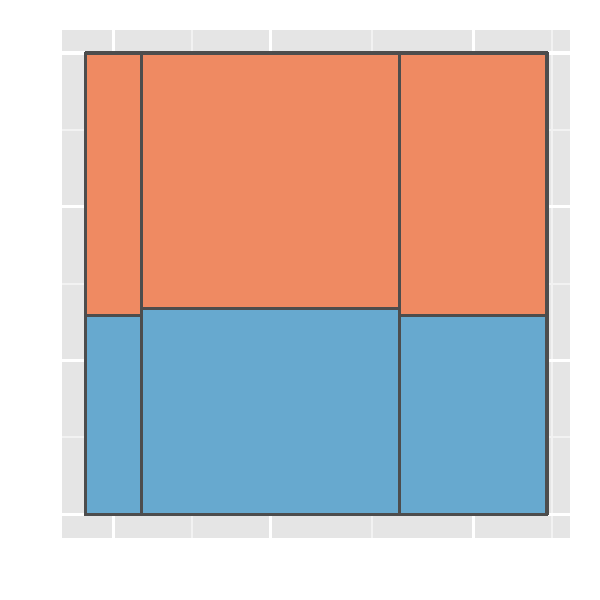
\includegraphics[width=0.25\linewidth]{hs-vs-cartesian}

    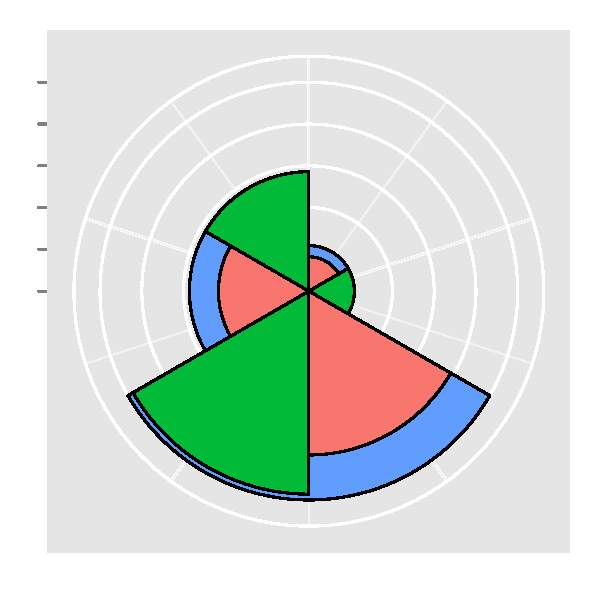
\includegraphics[width=0.25\linewidth]{hb-vb-polar}%
    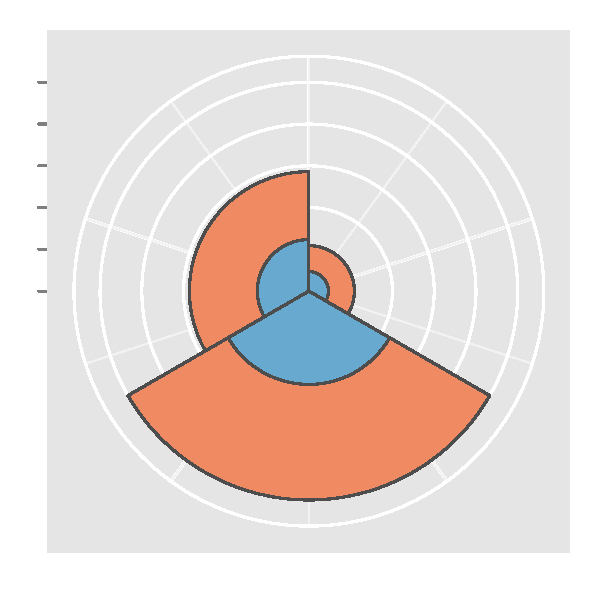
\includegraphics[width=0.25\linewidth]{hb-vs-polar}%
    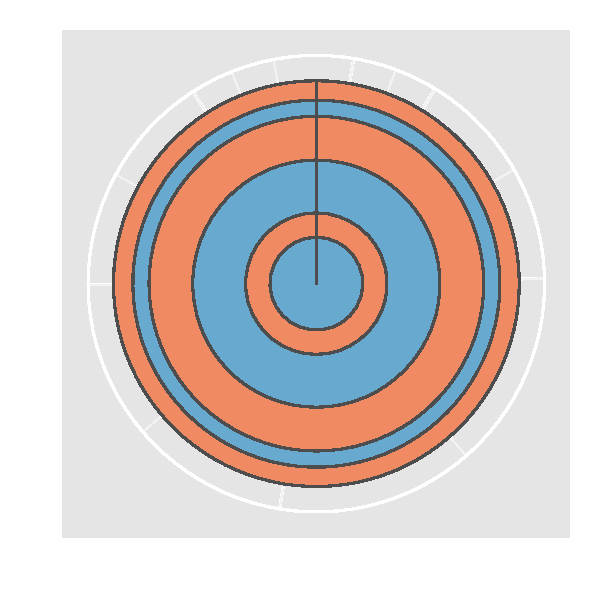
\includegraphics[width=0.25\linewidth]{hs-hs-polar}%
    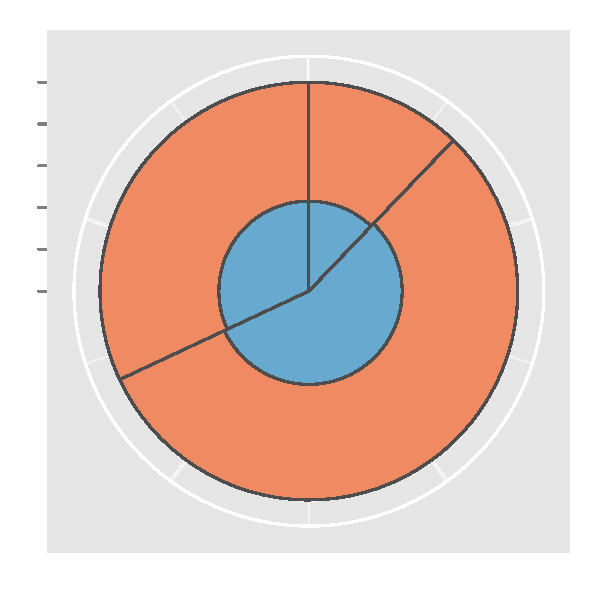
\includegraphics[width=0.25\linewidth]{hs-vs-polar}
  \caption{}
  \label{fig:polar}
\end{figure}

Circular treemaps of \citet{wetzel:2008} which use circles instead of rectangles, but is not space filling because you can not tile a circular region with circles. The radial displays of \citet{stasko:2000} deliberately keep the radius constant in order to relatively highlight the lower levels.  Similarly so does the fanlens of \citet{lou:2007}

Other non-rectangular treemaps have been proposed, such as the space-filling curve approach of \citep{wattenberg:2005}, or the voronoi treemaps of \citep{wattenberg:2005}, but because of the perceptual difficultly of comparing areas of arbitrary polygons, these approaches tend to be attractive rather than useful.

\section{Margining}
\label{sec:margining}

Mathematically defining margining operation.


\section{Connection with log-linear models}


\section{Variations}
\label{sec:variations}

% Pseudo 2d, where you take a long 1d structure and wrap it into 2d.
% 
% Pseduo 1d, where you make a new variable from multiple variables.


\subsection{Weighting}
\label{sub:weighting}

We have assumed the probabilities represent counts, but without loss of generality we can use any set of non-negative, additive weights instead.  Some of the applications of such weighted plots are described in \citet{unwin:2007}.  Include a brief summary here.

\subsection{Continuous data}
\label{sub:continuous_data}

These techniques can also be used with continuous data, if the data is binned to create a categorical variable. This gives rise to the histogram and spinogram, analogues of the bar chart and spine chart respectively. A long standing tradition is that no gaps are displayed between adjacent rectangles when used for originally continuous data. Two examples are shown in Figure \ref{fig:cont-examples}.

\begin{figure}[htbp]
  \begin{center}
  \end{center}
  \caption{Area plots of originally continuous data}
  \label{fig:cont-examples}
\end{figure}

Give a few examples of non-traditional continuous-categorical plots.  Fluctuation diagram for exploring joint 2d distribution.  Mosaic for conditional.  Age and year distribution.  

Cat + continuous.

\subsection{Nested data}
\label{sub:nested_data}

We distinguish nested data from crossed data by the number of interactions with missing values.  Completely crossed data contains every combination of all variables.  Nested data contains 

Aka sparse vs. dense.

It is not always possible to determine nested data from inspection of the data alone, but may need knowledge of the data collection.  For example, if a survey of teachers within schools was performed, and each teacher was identified by a identifier unique within a school, it might look like the data was only missing a few combinations, when in fact it is meaningless.  

Or when you have a hierarchy.

Example dataset

Possibilities: create new variable which is interaction of nested vars, or drop missings/zeros.  Treemaps deal almost exclusively with nested data.

\section{Labelling}
\label{sec:legends}

Labelling these plots is particularly challenging.  Future work!

\begin{itemize}
  \item Additional info 
  \begin{itemize}
    \item colour (map of the market)
    \item texture (sieve plots)
    \item photographs
    \item text (tables)
    \item embedded plots (time series in lab escape)
  \end{itemize}
  
  \item Display of hierarchy
  \begin{itemize}
    \item Spacing / borders
    \item Shading
    \item Cascading
    \item Labelling
  \end{itemize}
\end{itemize}

\section{Conclusions} % (fold)
\label{sec:conclusions}

% section conclusions (end)

% bibtool -x product-graphics -o references.bib
\bibliography{references}
\end{document}
